\documentclass[runningheads]{llncs}

\usepackage{graphicx}


\begin{document}

% \thanks{Supported by organization x.}
\title{Paper Title}
\author{First Author\inst{1} \and
Second Author\inst{1}
}
%\authorrunning{F. Author et al.}

\institute{Departamento de Informática da Faculdade de Ciências da Universidade de Lisboa
\email{\{fcXXXX,fcYYYY\}@alunos.fc.ul.pt}}

\maketitle

\begin{abstract}
The first sentence of an abstract should clearly introduce the topic of the paper so that readers can relate it to other work they are familiar with. However, an analysis of abstracts across a range of fields show that few follow this advice, nor do they take the opportunity to summarize previous work in their second sentence. A central issue is the lack of structure in standard advice on abstract writing, so most authors don’t realize the third sentence should point out the deficiencies of this existing research. To solve this problem, we describe a technique that structures the entire abstract around a set of six sentences, each of which has a specific role, so that by the end of the first four sentences you have introduced the idea fully. This structure then allows you to use the fifth sentence to elaborate a little on the research, explain how it works, and talk about the various ways that you have applied it, for example to teach generations of new graduate students how to write clearly. This technique is helpful because it clarifies your thinking and leads to a final sentence that summarizes why your research matters.

\keywords{First keyword  \and Second keyword \and Another keyword.}
\end{abstract}
%
%
%
\section{Introduction}


The introduction should set the context for your project. Why is this topic relevant?

You should also define the scope of your project. You could design a software artifact that would end poverty and famine, but that is not realistic.

For example, this document describes the structure your paper should have. Despite using the LNCS LaTeX template \footnote{LNCS is the official template for Europar 2019, in case you are interested.}, the formatting template is not relevant, only the content structure is relevant.

Finally, you should define the goals of your project. For instance,

\begin{itemize}
	\item To propose a method for the parallelization of Genetic Algorithms
	\item An implementation of such algorithm
	\item The experimental evaluation of such method, with comparison with a sequential alternative.
\end{itemize}


\section{Background}

This is an optional section, as it depends on your project. In projects where a given specific knowledge is required to understand the article, you should give a brief introduction of the required concepts. In the case of genetic algorithms, you should present the basic algorithm in this section.


\section{Approach}

In this section, you should present your approach. Notice that an approach may be different than an implementation. An approach should be generic and ideally applied for different machines, virtual machines or languages. You should present algorithms or generic diagrams explaining the approach.

\section{Implementation Details}

In this section you can talk about details of how you implemented your approach. Depending on the detail of your approach, this might be an optional section.

As an example, I would detail how I implemented the phaser in the genetic algorithm, or how I implemented parallel mergesort on ForkJoin. Another aspect could be how to organize your arrays to minimize overhead in recursive calls.


\section{Evaluation}

\subsection{Experimental Setup}

In this section you should describe the machine(s) in which you are going to evaluate your system. Select the information that is relevant.


\subsection{Results}

In this section you should present the results. Do not forget to explain where the data came from. 

You should include (ideally vectorial) plots, with a descriptive caption. Make sure all the plots (Like Figure~\ref{fig1} are well identified and axis and metrics are defined.

\begin{figure}[htbp]
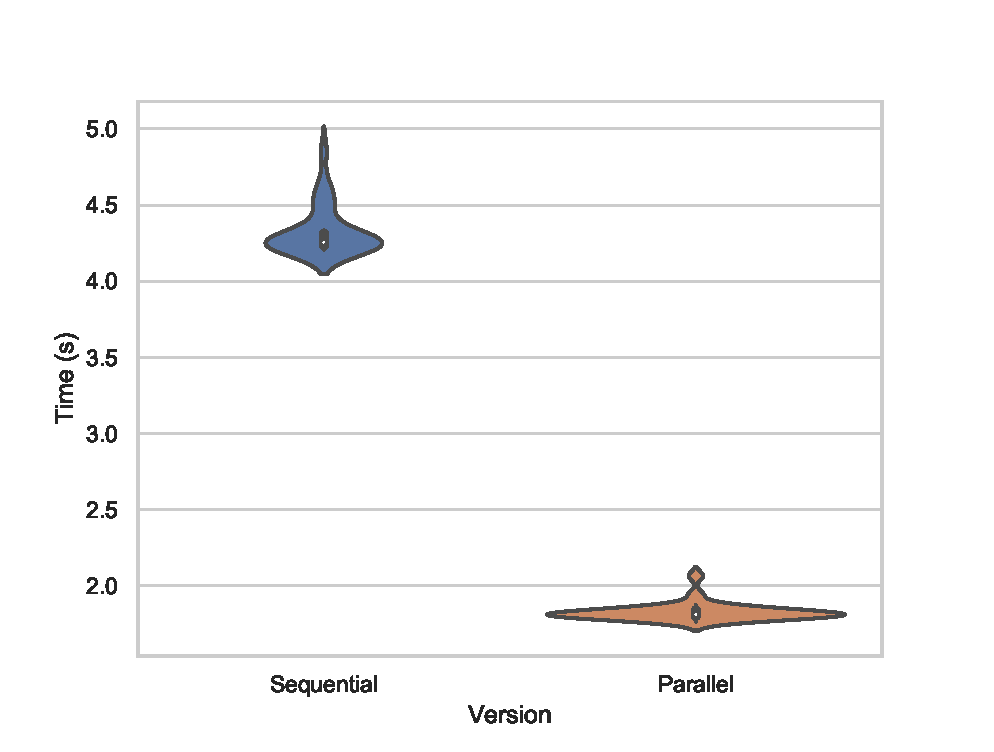
\includegraphics[width=\textwidth]{code/performance.eps}
\caption{Comparison of the performance of sequential and parallel versions of the algorithm.} \label{fig1}
\end{figure}


\subsection{Discussion}

Here you should discuss the results on a high level. For instance, based on our results, the parallelization of the merge-sort is relevant as no other parallel work occurs at the same time, and the complexity $O(N log(N))$ can have a large impact when the number of individuals is high.

\section{Related Work}

This section can be either the second one, or the second-to-last. In the case where knowledge of other competing works is required, it could come before. But if you are confident on what you did, it should appear at the end, where you can compare existing works against yours. An example is below:

Chu and Beasley proposed a Genetic Algorithm for the Multidimensional Knapsack Problem \cite{DBLP:journals/heuristics/ChuB98}. This work introduces a heuristic as a repair operator. Our work makes no optimization with regards to the problem domain, making it more generic and supporting other problems.


When using BibTeX references, I suggest using DBLP\footnote{\url{https://dblp.org}}, leaving Google Scholar as a backup, since DBLP has more correct and detailed information about research papers.

\section{Conclusions}

Here you should resume the major conclusions taken from discussion. Ideally, these should align with the objectives introduced in the introduction.


You should also list the future work, i. e., tasks and challenges that were outside your scope, but are relevant.

\section*{Acknowledgements}

First Author wrote the part of the program implemented the phasers. Second Author implemented the MergeSort in parallel. 

Both authors wrote this paper, with First Author focusing on the introduction, related work and conclusions while the Second Author focused on approach and evaluation.

Each author spent around 30 hours on this project.

\bibliographystyle{splncs04}
\bibliography{bibliography}

\end{document}
